\documentclass[12pt,letterpaper]{article}
\usepackage[spanish]{babel}
\usepackage[utf8]{inputenc}
\usepackage{graphicx}
\usepackage{pst-pdf}
\usepackage{amssymb}
\usepackage{hyperref}
\usepackage{listings}
\usepackage{biblatex}
\addbibresource{tarea_5.bib} 
\title{{Programacion estructurada.}}
\author{Daniel Reyes Barrera}
\date{23 de noviembre de 2020}

\begin{document}
\maketitle

\abstract{En este documento se han resuelto algunos problemas computacionales utilizando las herramientas aprendidas en la clase 5 – Programaci\'on estructurada del curso de programaci\'on C++, como son Modularizaci\'on, m\'etodos y funciones las cuales nos proporcionan un mejor uso para un bloque recurrente de instrucciones.



\section{Ejercicio 1.}

Escriba un programa que imprima un men\'u para seleccionar un tipo de
gura geom\'etrica de la siguiente forma:
\begin{figure}[ht!]
  \centering
  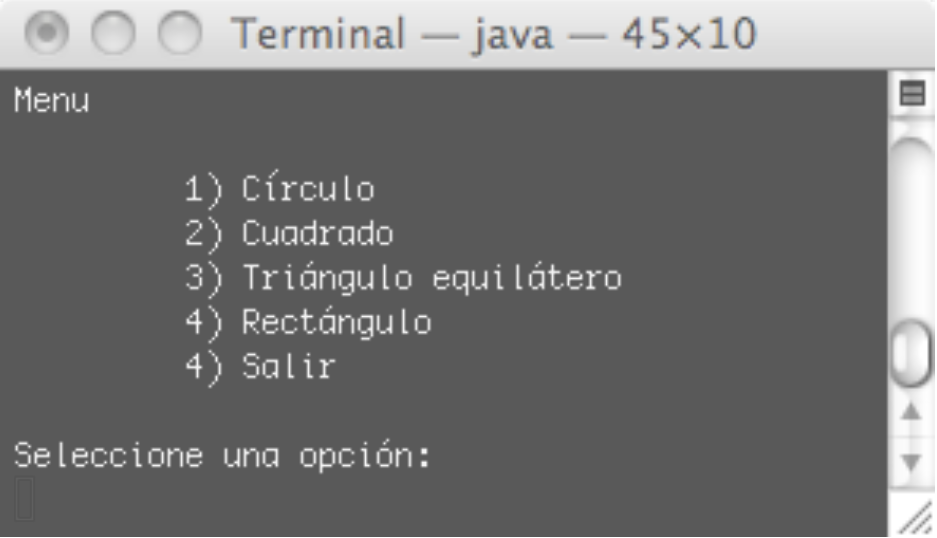
\includegraphics[width=0.6\textwidth]{figures/captura}
  \label{fig:bisiesto}
\end{figure}

El usuario debe seleccionar una opci\'on y el programa debe calcular el \'area y per\'imetro de la opci\'on seleccionada. Programe cada opci\'on en un m\'etodo independiente. El programa debe regresar al menu principal hasta que el usuario seleccione la opci\'on salir.

\subsection{Problema computacional.}
\textbf{Objetivo:} Dado un n\'umero entero como año determinar si es un año bisiesto o no.

\textbf{Entrada:} Un n\'umero entero mayor que 0 representando un año.

\textbf{Salida:} La respuesta de si el n\'umero dado es un año bisiesto o no.

\subsection{Algoritmo.}
Para solucionar el problema computacional, partimos de la definici\'on de un año bisiesto. Un año se denomina bisiesto si es m\'ultiplo de 4, a excepci\'on de que s\'i es m\'ultiplo de 100 tambi\'en y no de 400 entonces no es bisiesto, por tanto necesitaremos utilizar el condicional \texttt{if-else} para validar que se cumplan las condiciones para que el año sea bisiesto o no.


El código fuente está disponible en mi repositorio de git hub. \cite{url:basilea}

\subsection{Instancia del problema.}
Como prueba de escritorio, se seleccionaron las siguientes instancias del problema. Entrada: 44, 200, 800 y 122423. La salida del programa se observa en la Figura \ref{fig:bisiesto}.
\begin{figure}[ht!]
  \centering
  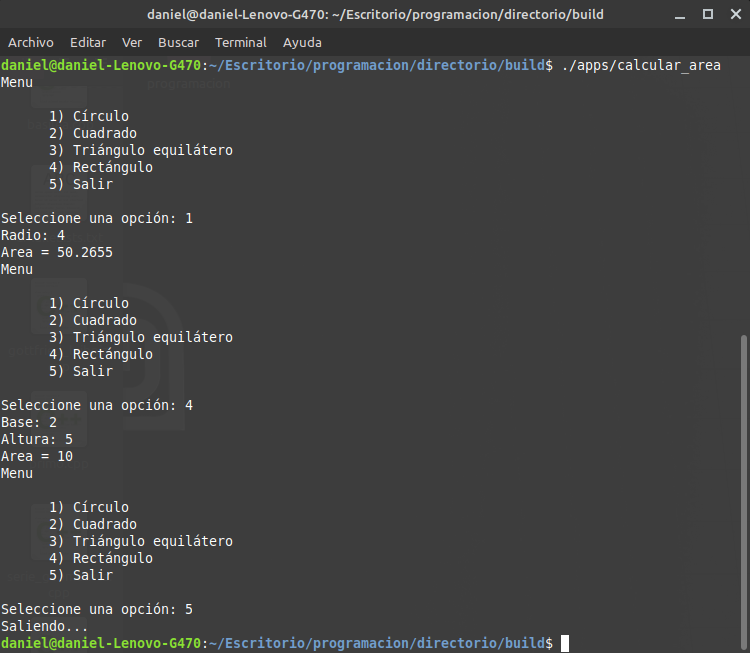
\includegraphics[width=0.8\textwidth]{figures/calcular_area}
  \caption{Ejecución de algunas instancias del problema.}
  \label{fig:bisiesto}
\end{figure}

\section{Ejercicio 2.}

El m\'aximo com\'un divisor de dos enteros es el entero m\'as grande que puede dividir a cada uno de los dos n\'umeros. Programe el algoritmo para calcular el m\'aximo com\'un divisor en un m\'etodo independiente.

\subsection{Problema computacional.}
\textbf{Objetivo:} Dado un n\'umero entero como año determinar si es un año bisiesto o no.

\textbf{Entrada:} Un n\'umero entero mayor que 0 representando un año.

\textbf{Salida:} La respuesta de si el n\'umero dado es un año bisiesto o no.

\subsection{Algoritmo.}
Para solucionar el problema computacional, partimos de la definici\'on de un año bisiesto. Un año se denomina bisiesto si es m\'ultiplo de 4, a excepci\'on de que s\'i es m\'ultiplo de 100 tambi\'en y no de 400 entonces no es bisiesto, por tanto necesitaremos utilizar el condicional \texttt{if-else} para validar que se cumplan las condiciones para que el año sea bisiesto o no.


El código fuente está disponible en mi repositorio de git hub. \cite{url:basilea}

\subsection{Instancia del problema.}
Como prueba de escritorio, se seleccionaron las siguientes instancias del problema. Entrada: 44, 200, 800 y 122423. La salida del programa se observa en la Figura \ref{fig:bisiesto}.
\begin{figure}[ht!]
  \centering
  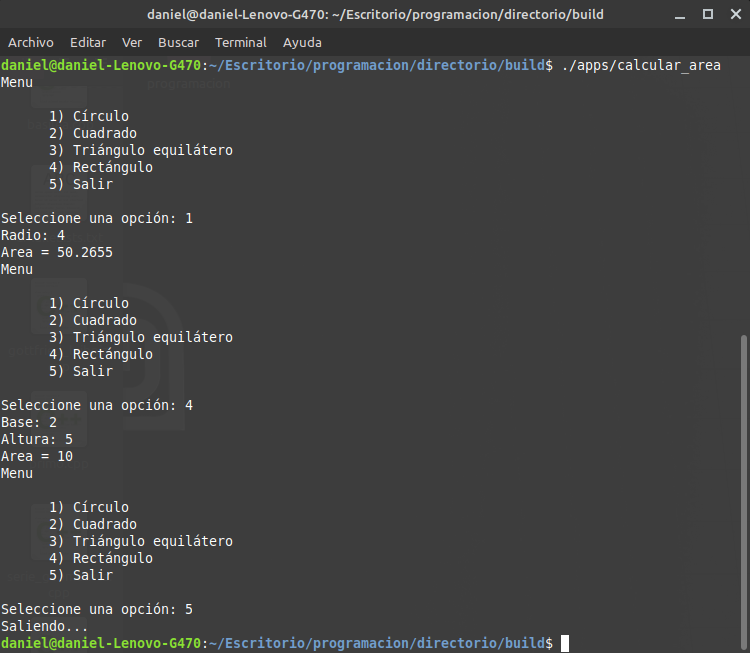
\includegraphics[width=0.8\textwidth]{figures/calcular_area}
  \caption{Ejecución de algunas instancias del problema.}
  \label{fig:bisiesto}
\end{figure}

\section{Ejercicio 3.}

Programe el algoritmo para determinar si el n\'umero es pal\'indromo y el algoritmo para validar la entrada en m\'etodos independientes.
Sugerencia: Haga uso de los operadores m\'odulo y divisi\'on para separar el n\'umero tecleado en unidades, decenas, centenas, etc.

\subsection{Problema computacional.}
\textbf{Objetivo:} Dado un n\'umero entero como año determinar si es un año bisiesto o no.

\textbf{Entrada:} Un n\'umero entero mayor que 0 representando un año.

\textbf{Salida:} La respuesta de si el n\'umero dado es un año bisiesto o no.

\subsection{Algoritmo.}
Para solucionar el problema computacional, partimos de la definici\'on de un año bisiesto. Un año se denomina bisiesto si es m\'ultiplo de 4, a excepci\'on de que s\'i es m\'ultiplo de 100 tambi\'en y no de 400 entonces no es bisiesto, por tanto necesitaremos utilizar el condicional \texttt{if-else} para validar que se cumplan las condiciones para que el año sea bisiesto o no.


El código fuente está disponible en mi repositorio de git hub. \cite{url:basilea}

\subsection{Instancia del problema.}
Como prueba de escritorio, se seleccionaron las siguientes instancias del problema. Entrada: 44, 200, 800 y 122423. La salida del programa se observa en la Figura \ref{fig:bisiesto}.
\begin{figure}[ht!]
  \centering
  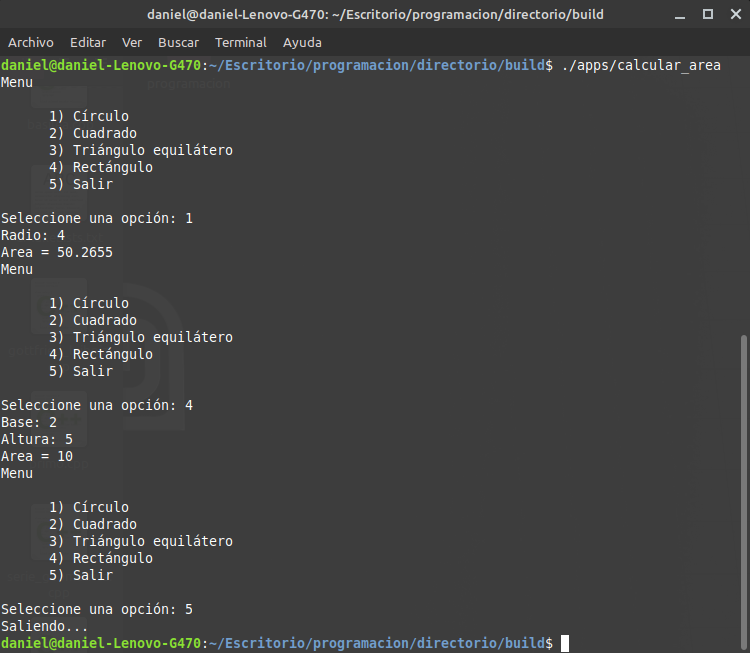
\includegraphics[width=0.8\textwidth]{figures/calcular_area}
  \caption{Ejecución de algunas instancias del problema.}
  \label{fig:bisiesto}
\end{figure}

\section{Ejercicio 4.}

Programe el algoritmo de Schrage para generar n\'umeros pseudo-aleatorios
entre $0$ y $m$.
El j-\'esimo elemento de la sucesi\'on de n\'umeros pseudo-aleatorios, denotado por $I_j$ , se calcula con la siguiente ecuaci\'on:
$$ I_j = a(I_{j-1} mod \ m) $$
$$I_{j}=\left\lbrace\begin{array}{c} a(I_{j-1} mod \ q)-r[I_{j-1} /q] \ \ \ si \ a(I_{j-1} mod \ q )-r[I_{j-1}/q > 0] \\ a(I_{j-1} mod \ q)-r[I_{j-1} /q] + m \ \ \ \ \ \ \ \ en \ otro \ caso \ \ \ \ \ \ \ \ \  \ \ \ \ \ \end{array}\right.  $$

donde $a = 75$, $m = 2^31-1$, $q = 127773$, $r = 2836$ y $I_0$ es la semilla del generador, cuyo valor se deja a criterio del programador. Los corchetes indican que el resultado de la divisi\'-on se trunca para obtener solamente la parte entera.


\subsection{Problema computacional.}
\textbf{Objetivo:} Dado un n\'umero entero como año determinar si es un año bisiesto o no.

\textbf{Entrada:} Un n\'umero entero mayor que 0 representando un año.

\textbf{Salida:} La respuesta de si el n\'umero dado es un año bisiesto o no.

\subsection{Algoritmo.}
Para solucionar el problema computacional, partimos de la definici\'on de un año bisiesto. Un año se denomina bisiesto si es m\'ultiplo de 4, a excepci\'on de que s\'i es m\'ultiplo de 100 tambi\'en y no de 400 entonces no es bisiesto, por tanto necesitaremos utilizar el condicional \texttt{if-else} para validar que se cumplan las condiciones para que el año sea bisiesto o no.


El código fuente está disponible en mi repositorio de git hub. \cite{url:basilea}

\subsection{Instancia del problema.}
Como prueba de escritorio, se seleccionaron las siguientes instancias del problema. Entrada: 44, 200, 800 y 122423. La salida del programa se observa en la Figura \ref{fig:bisiesto}.
\begin{figure}[ht!]
  \centering
  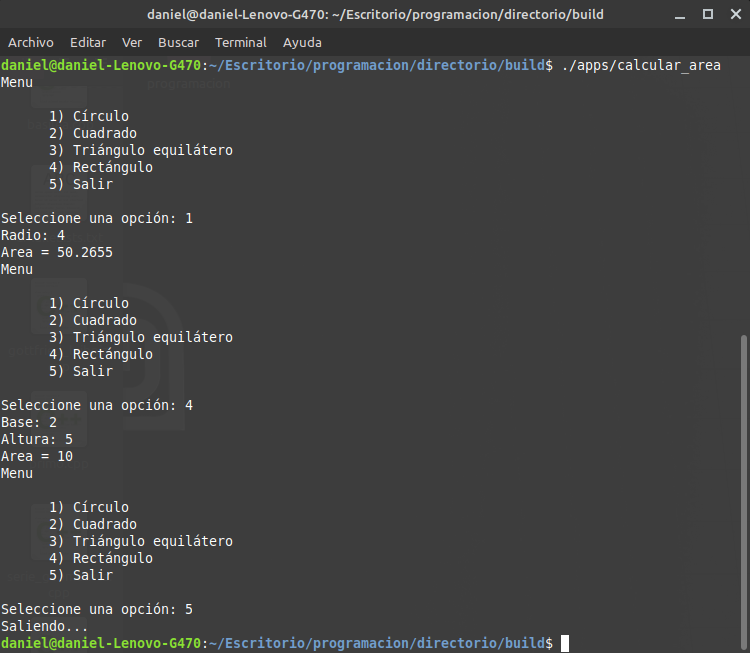
\includegraphics[width=0.8\textwidth]{figures/calcular_area}
  \caption{Ejecución de algunas instancias del problema.}
  \label{fig:bisiesto}
\end{figure}





\section{Conclusiones.}
Las Estructura de control condicionada ( \texttt{if-else} o \texttt{switch-case}), estructuras de control por repetici\'on (\texttt{for}, \texttt{while}, \texttt{do-while}) pueden resolver muchos problemas en el cual se requieran ciclos o codiciones, pero si incluimos los array los problemas abarcables son innumerables.

\printbibliography 


\end{document}
